\subsection{Fonction chromatique $P_G(k)$}
Le nombre de manières de colorier un graphe est le produit des nombres de façons de colorier chaque arc.
\begin{itemize}
\item Si le graphe $G$ est complet, on aura $k$ couleurs possibles pour le premier sommet, $(k-1)$ pour le deuxième, etc\ldots (Le graphe G étant complet, la couleur du premier sommet est nécessairement exclu des autres sommets).

Le $n$\^{ième} sommet pourra être colorié de $k-(n-1)$ manières. D'où :
\[ P_{K_n}(k)=\prod_{i=0}^{n-1}(k-i) \]

\item Si $G$ est vide, la coloration d'un sommet ne contraint pas la coloration des autres sommets. On obtient alors :
\[ P_{\overline{K_n}}(k)=k^n \]
\end{itemize}

\subsection{Nombre chromatique $\chi(G)$}
On l'appelle "nombre chromatique" de $G$: $\chi(G)$ étant, par définition, le nombre minimum de couleurs nécessaires pour colorier $G$, si $k < \chi(G)$ alors le graphe $G$ ne peut pas être colorié par $k$ couleurs. Si $k \geq \chi(G)$ alors il doit y avoir au moins une manière de colorier $G$, celui utilisant $\chi(G)$ couleurs.

On a donc :
\begin{displaymath}
	P_G(k) \left\{ \begin{array}{ll}
	=0 & \textrm{si $k < \chi(G)$} \\
	\geq 1 & \textrm{sinon}
	\end{array} \right.
\end{displaymath}

\subsection{Décomposition de $P_G$}
Montrons d'abord que la propriété est vraie pour tout graphe complet $K_n$. Pour commencer on remarque que, pour tout arrête $e$:

\begin{itemize}
\item $K_{n\backslash e}$ est exactement $K_{n-1}$, et donc: 

\[ P_{K_n\backslash e}(k) = P_{K_{n-1}} = \prod_{i=0}^{n-2}(k-i) \]


\item Soit $e = (a,b)$. On peut supposer (sans perte de généralité) que $b$ est considéré en dernier lors de la coloration de $K_n$, donc qu'il lui reste $k-(n-1)$ couleurs. Pour colorier $K_{n-e}$ on aura un choix de plus pour lui, à savoir la couleur de $a$, donc $k-(n-2)$ en totale. De ce fait:

\[ P_{K_n-e}(k) = P_{K_{n-1}}(k)(k-(n-2)) = (\prod_{i=0}^{n-2}(k-i))(k-(n-2)) \]
\end{itemize}

On a donc très clairement:
\begin{eqnarray*}
P_{K_n-e}(k) -  P_{K_n\backslash e}(k) &=& (\prod_{i=0}^{n-2}(k-i))(k-(n-2)) - \prod_{i=0}^{n-2}(k-i)\\
&=& \prod_{i=0}^{n-2}(k-i)(k-(n-1))\\
&=& \prod_{i=0}^{n-1}(k-i)\\
&=& P_{K_n}(k)
\end{eqnarray*}
Tout graphe de rang $n$ pouvant se générer à partir de $K_n$ (en enlevant des arrêtes) on cherchera à prouver que la suppression d'arrête conserve notre propriété. Autrement dit on aimerait montrer que pour tout graphe $G$ et tout arrête $a$ de celui-ci:

\begin{eqnarray*}
&&P_G(k) = P_{G-e}(k) - P_{G \backslash e}(k) \\
&\Rightarrow&  P_{G-a}(k) = P_{G-e-a}(k) - P_{G \backslash e-a}(k)
\end{eqnarray*}

On supposera évidemment que $a$ et $e$ sont distinctes. 

TODO FINISH

\subsection{Polynôme chromatique ?}
Soit $H$ un prédicat tel que :
\begin{displaymath}
	H(m) = \left\{ \begin{array}{ll}
	\top & \textrm{si $\forall$ $G$, graphe de $m$ arrêtes ou moins, $P_G(k)$ est polynomiale.} \\
	\bot & \textrm{sinon.}
	\end{array} \right.
\end{displaymath} 
\begin{itemize} 
\item Nous rappellons que $P_{\overline{K_n}}(k)=k^n$, donc $H(0)$ est vraie. 
\item Supposons $\exists m \in \mathbb{N}$ $|$ $H(m)$ l'est également. Ajoutons l'arc $a$ à $G$. $G_{m+e}$ est un graphe à $(m+1)$ arrêtes :

\[ P_{G_{m+z}} = P_{G_{m+e}-e} - P_{G_{m+e} \backslash e} \]

Clairement $P_{G_{m+1}-e}$ et $P_{G_{m+1} \backslash e}$ ont $(m+1)-1 = m$ arrêtes. Or par hypothèse de recurrence $H(m)$ est vraie,
$P_{G_{m+1}}$ est la différence entre deux polynomiales, donc est polynomiale lui-même. On a donc $H(m+1)$.
\item On vient de montrer $(H(0) \wedge (H(m) \Rightarrow H(m+1)))$. Par récurrence on a donc $H(m)$ vrai $\forall m \in \mathbb{N}$. 

\end{itemize} 

\subsection{Application de la décomposition}
Utilisons la formule trouvée au point précédent, et admettons que pour $P_n$ une chaîne de taille $n$ on a :
\[ P_{P_n}(k) = k(k-1)^{n-1} \]

Prenons $A$ le graphe initial :
\begin{eqnarray*}
P_A(k) & = & P_B(k) - P_C(k) \\
&=& \big(P_D(k)-P_E(k)\big)-\big(P_F(k)-P_{P_3}(k)\big)\\
&=& \Big[\big(P_{P_5}(k)-P_{P_4}(k)\big)-\big(P_{P_4}(k)-P_{P_3}(k)\big)\Big]-\Big[\big(P_{P_4}(k)-P_{K_3}(k)\big)-P_{P_3}(k)\Big]\\
&=& P_{P_5}(k)+2P_{P_3}(k)-P_{K_3}(k)+3P_{P_4}(k)\\
&=& k(k-1)^4 +2k(k-1)^2+k(k-1)(k-2)-3(k-1)^3 \\
&=& k(k-1)\big[(k-1)^3+z(k-1)+(k-z)-3(k-1)^2\big]\\
&=& (k^2-k)\Big[(k-1)^2\big((k-1)-3\big)+3k -4 \Big]\\
&=& (k^2-k)[k^3-6k^2+12k-8]\\
&=& k^5-7k^4+18k^3-20k^3+8k
\end{eqnarray*}
Où :

$A$ : \raisebox{-0.5\height}{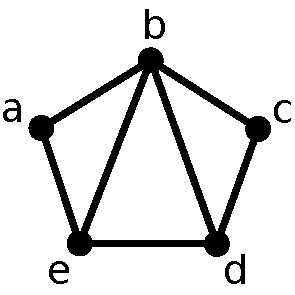
\includegraphics[width=2cm]{files/gAex1.pdf}}

\begin{tabular}{llcll}
$B = A-(e,d) $ : & \raisebox{-0.5\height}{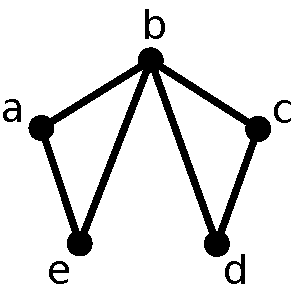
\includegraphics[width=2cm]{files/gBex1.pdf}} & et & $C = A\backslash(e,d)$ : & \raisebox{-0.5\height}{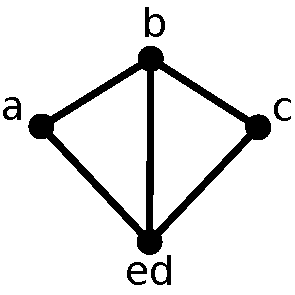
\includegraphics[width=2cm]{files/gCex1.pdf}} \\
$D = C-(a,b)$ : & \raisebox{-0.5\height}{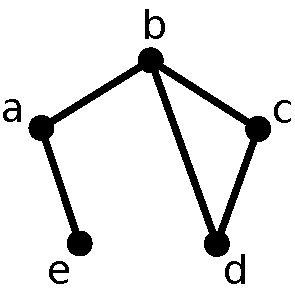
\includegraphics[width=2cm]{files/gDex1.pdf}} & et & $E = C\backslash(e,b)$ : & \raisebox{-0.5\height}{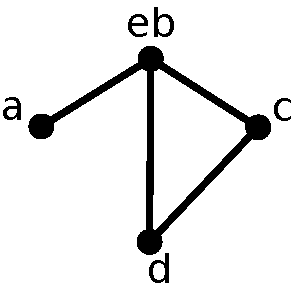
\includegraphics[width=2cm]{files/gEex1.pdf}} \\
$F = C-(b,ed)$ : & \raisebox{-0.5\height}{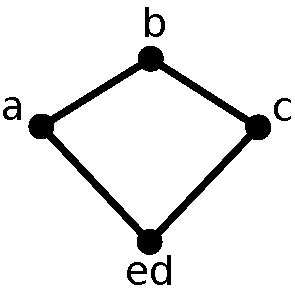
\includegraphics[width=2cm]{files/gFex1.pdf}}& et & $C \backslash(b,ed) = P_3$ : & \raisebox{-0.5\height}{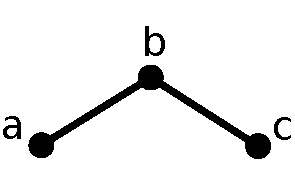
\includegraphics[width=2cm]{files/gC-ex1.pdf}}
\end{tabular}

\subsection{Particularités des polynômes chromatiques}
Nous cherchions à prouver que pour tout graphe $G$ à $n$ sommets et $m$ arrêtes, avec $C = \{c_i\}$ un ensemble de coéfficients naturelles (donc positives) : 
\[ P_G(k) = k^n - mk^{n-1} + \sum_{i = 2}^n \Big(\big(1 - 2(2\bmod{i})\big)(c_ik^{n-i})\Big) \]
On nomera $F_k(n,m,C)$ cette forme polynomiale particulière. Soit $H$ un prédicat tel que :
\[ H(n,m) \Leftrightarrow \forall{G(n,m)}, \hspace{1mm} \exists{C} \hspace{1mm} 
										| \hspace{1mm} P_G(k) = F(n, m, C) \]
On montrera par récurance que $H(n,m)$ est vrai pour tout $n$ et tout $m$ :
\begin{itemize}
\item \textbf{Sommets -- cas de base} \\
Pour $n = 1$ on a $P_G(k) = k$, donc $H(0,1)$ est vérifié.
\item \textbf{Sommets -- pas récursif} \\ Supposons qu'il existe un nombre de sommets $n_0$ et un nombre d'arrêtes $m_0$ tel que $H(m_0,n_0)$ soit vrai. Soit $G$ un graphe à $n_0$ sommets et $m_0$ arrêtes, et $G^+$ le graphe généré en reliant un nouveau sommet $s'$ à une selection de $n' \leq n_0$ sommets de $G$. On aura donc $(k-n')$ manières de colorier $s'$. De ce fait:
\[ P_{G^+}(k) = P_G(k)(k-n') \]
Où $P_G(k)$ est de la forme $F$. $P_G^+(k)$ est donc de la forme:
\begin{eqnarray*}
&&	F(n,m,C)(k-n')			\\
&=& F(n,m,C)k - n'F(n,m,C)	\\
\end{eqnarray*} 
\begin{itemize}
\item \textbf{Maintient des signes alternatifs} \\ 
Le fait de multiplier par $k$ "décale" les termes du polynomiale à gauche. Soustraire $n'F_k(n,m,C)$ retranche alors au coéfficient de chaque terme $n'$ fois celui de leur voisin de gauche, avec $0 \leq n' \leq n$. Or si le term est positive, ce fameux voisin de gauche est négative par hypothèse, donc son coéfficient augmentera. De même si le term est négative son coéfficient va diminuer. Les signes resteront donc alternatifs dans $P_G^+(k)$.
\item \textbf{Maintient de $k^n$} \\
$k^{n}$ deviendra $k^{n+1}$ dans $F_k(n,m,C)k$ et, n'aillant pas de voisin gauche dans $F_k(n,m,C)$, on ne lui retranchera rien. La propriété sur le terme de plus haut degré est donc maintenu.
\item \textbf{Maintient de $mk^{n-1}$} \\
Le terme $-mk^{n-1}$, aillant pour voisin gauche $k^n$, deviendra \[-mk^n - n'k^n = -(m+n')k^n \] $(m+n')$ étant le nombre d'arrêtes de $G^+$. La propriétée sur le second terme de plus haut degré est alors maintenu aussi.
\end{itemize}

\item \textbf{Arrêtes -- cas de base} \\
Pour $m = 0$ on a $G = \overline{K}_n$ et donc $P_G(k) = P_{\overline{K}_n}(k) = k^n$. Du coup $\forall n \in \mathbb{N^+}$, $H(0,n)$ est vrai.
\item \textbf{Arrêtes -- pas récursive} \\
Supposons qu'il existe un nombre d'arrêtes $m_0$ tel que pour tout $m \leq m_0$ et tout $n$ on a $H(m_0,n)$. Soit $G$ un graphe à $m_0 + 1$ arrêtes. D'après la formule du question $3$ on a donc:
\begin{eqnarray*}
P_G(k) &=& P_{G-e}(k) - P_{G \backslash e}(k)	\\
		&=& A - B								\\	
\end{eqnarray*}
Où $A$ et $B$ sont de la forme $F_k$. $P_G(k)$, lui, est donc de la forme:
\[ F_k(n,m-1,C') - F_k(n-1,m-1,C'') \]

\end {itemize}

\subsection{Polynôme chromatique de $K_{1,5}$}
$K_{1,5}$ étant un arbre, on aura $k$ choix de coloration pour la racine, peu importe le choix de celle-ci, et $k-1$ pour les autres, car chacun qu'on considère sera relié à exactement une autre déjà colorié. En totale ça nous fait donc:
\begin{eqnarray*}
P_{K_{1,5}}(k) 	& = & k(k-1)^5 \\
				& = & k{((k-1)^2)}^2(k-1)	\\
				& = & k(k^2 - (2k - 1))^2(k-1)	\\
				& = & (k^5 - 4k^4  + 6k^3 - 4k^2 + k)(k-1)  \\
				& = & k^6 - 5k^5  + 10k^4 - 10k^3 + 5k^2 - k	\\ 
\end{eqnarray*}

\subsection{Coloration de graphes non-connexes}
La coloration de chaque composante connexe $C_i$ n'influx pas sur celui des autres. Du coup le nombre de manières de colorier un graphe entier est le produit des polynômes chromatiques de ses composantes connexes:
\begin{eqnarray*}
G = \bigcup_{i=0}^n C_i & \Rightarrow & P_G(k)=\prod_{i=0}^n P_{C_i}(k) \\
\end{eqnarray*}

\subsection{Coloration d'arbres}
Supposons qu'on ait un graphe $G$ tel que $P_G(k) = k(k-1)^{n-1}$ :
\begin {itemize}
\item Intuitivement ceci veut dire qu'on a $k$ choix de couleurs pour le premier sommet colorié, puis $(k-1)$ pour chacun des $(n-1)$ autres. Du coup chaque sommet, lors de sa coloration, ne doit être en contact qu'avec un seul sommet déjà colorié. Ceci n'est possible que dans un graphe sans cycle, car même avec un seul cycle on aura au plus $k(k-1)^{n-2}(k-2) < k(k-1)^{n-1}$ colorations différentes.
\item De même si $G$ est une forêt, même s'il n'est composé que de deux composantes connexes, il devraient y avoir au moins $k^2(k-1)^{n-2} > k(k-1)^{n-1}$ colorations possibles.
\end {itemize}
On a donc $G$ connexe et sans cycle: c'est la définition même d'un arbre.

\subsection{$k^5 - 4k^4 + 6k^3 - 4k^2 + k$}
Grace aux dévelopments précédentes (questions $7$ et $12$) on reconnait:
\begin{eqnarray*}
&&		k^5 - 4k^4 + 6k^3 - 4k^2 + k 	\\	
&=&		k(k-1)^4						\\
&=&		P_{P_5}(k)						\\
\end{eqnarray*}
Notre premier exemple sera donc $P_5$ le chemin de taille $5$. Ensuite d'après la propriété de la question $6$ nous ne cherchions que des graphes aillant $5$ sommets et $4$ arrêtes, et d'après celle de la question $9$ ils doivent en plus être arbres. Nous proposons donc le graphe étoile $S_5 = K_{1,4}$ ainsi que l'arbre à $5$ sommets dont la particularité est d'être sans particularité:

\begin{center}
$S_5$ : \raisebox{-0.5\height}{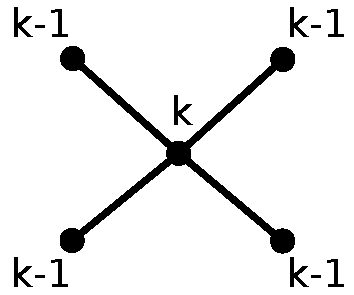
\includegraphics[width=2cm]{files/s5ex1.pdf}} \hspace{3cm}
$A_5$ : \raisebox{-0.5\height}{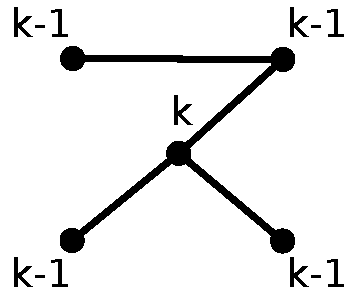
\includegraphics[width=2cm]{files/a5ex1.pdf}}
\end{center}

\subsection{Polynôme chromatique de $K_{2,5}$}
Nous avions déjà calculé le polynôme chromatique de $K_{1,5}$ :
\[ P_{K_{1,5}}(k) = k^6 - 5k^5  + 10k^4 - 10k^3 + 5k^2 - k \]
Or $K_{2,5}$ se construit à partir de $K_{1,5}$ par l'ajout d'un sommet relié au $5$ de la partition majoritaire. Ce nouveau sommet pourra être colorié de $(k-5)$ manières, car seront interdis les couleurs de ses $5$ voisins. On a donc :
\begin{eqnarray*}
P_{K_{2,5}} & = &	(P_{K_{1,5}}(k))(k-5)								\\
			& = & 	(k^6 - 5k^5  + 10k^4 - 10k^3 + 5k^2 - k)(k-5)		\\	
			& = &	k^7 - 10k^6 + 35k^5 - 60k^4 + 55k^3 - 26k^2 + 5k	\\
\end{eqnarray*}

\subsection{Polynômes chromatiques de $C_4$ et $C_5$}
\begin {itemize}
\item Pour calculer $P_{C_4}$, commençons par constater que $C_3 = K_3$ :
\begin{eqnarray*}
P_{C_4}(k)	& = &	P_{P_4}(k) - P_{K_3}(k)				\\
			& = & 	k(k-1)^3 - k(k-1)(k-2)				\\
			& = & 	(k^2 - k)((k-1)^2 - (k-2))			\\
			& = &	(k^2 - k)(k^2 - 3k + 3)				\\
			& = & 	k^4 - 4k^3 + 6k^2 - 3k				\\			
\end{eqnarray*}
\item On peut alors utiliser $P_{C_4}$ pour calculer $P_{C_5}$ :
\begin{eqnarray*}
P_{C_5}(k)	& = &	P_{P_5}(k) - P_{C_4}(k)				\\
			& = & 	k(k-1)^4 - k^4 -4k^3 + 6k^2 - 3k	\\
			& = &	k^5 - 5k^4 + 10k^3 - 10k^2 + 4k		\\ 
\end{eqnarray*}
\end {itemize}

\subsection{Coloration de cycles}
cycles générales

\subsection{Coloration de graphes bipartis complets}
graphe bipartie générale